\documentclass[12pt]{ieeetj}
% Packages
\usepackage{graphicx}
\usepackage{amsmath}
\usepackage{hyperref}
\usepackage{setspace}
\usepackage{listings}
\usepackage{xcolor}  % Include xcolor for text color
\usepackage{abstract}
\usepackage{float}

% Customize section font size

\lstset{
  literate={\_}{{\_}}{1},   % Replace _ with the literal \_
  basicstyle=\scriptsize\ttfamily,      % Optional: Set typewriter font for listings
  breaklines=true,            % Enable line breaking for long lines
  postbreak=\mbox{\textcolor{red}{$\hookrightarrow$}\space}, % Optional: indicate line break
  literate={|}{{\textbar}}1 {0}{{0}}1 {>}{{\textgreater}}1 {\_}{{\_}}1,
  escapechar=\%             % Optional: Set an escape character if needed
}
% Title and Author (adjust the spacing as needed)
\title{\LARGE \textbf{Quantum Networking: Explore QKD and quantum internet}}
\author{}
\date{\large On: \today}
\def\seclogo{} 
% Begin Document
\begin{document}
\onecolumn
% Title Page
\makeatletter
\begin{titlepage}
\centering
\vspace* {1cm}
{ 
\includegraphics[width=6cm]{ELMEPA.png}}\\[1cm]

{\LARGE \textbf{Quantum Networking: Explore QKD and quantum internet}}\\[1cm]
Project for\\[1cm]

	Advanced Networks Master's program course\\[0.5cm]



	\textbf{Written By:} {Nikolaos Mouzakitis MTP321}\\[1cm]
\date{\large Date Last Edited: \today}
{\@date\\}
\end{titlepage}
\makeatother
% Abstract


	\begin{abstract}
	%\addcontentsline{toc} {chapter} {Abstract}

		Quantum networking represents a transformative advancement in secure communication,
		utilizing principles of quantum mechanics such as superposition, entanglement, no-cloning theorem for addressing
		vulnerabilities in widely adopted classical cryptographic systems, 
		with Quantum Key Distribution (QKD) and the quantum internet standing at its core.
		Unlike the classical systems, QKD makes use of certain mechanical principles
		from the field of quantum physics in order to theoretically guarantee unbreakable encryption schemes.
		In the early days of its rise, quantum internet promises a global network enabling unprecedented levels of
		secure communication, distributed quantum computing, and advanced scientific applications.
		Despite the progress, scalability remains a main bottleneck, alongside with the issues that leads into this scalability challenge. 
		Current quantum networks are constrained because of photon loss in fiber optic mediums, quantum gate losses and noise to quantum states
		are very fragile. All these behaviors introduce diffuculties for scaling quantum systems.
		In this project the current state of quantum networking is explored and simulations using QuTiP or
		experimental deployments on IBM’s quantum computers (IBMQ) are presented to study entanglement distribution,
		quantum teleportation, quantum state error correction and hybrid quantum-classical network communication.

	\end{abstract}
	
        \section{Introduction}

		Quantum networking stands as the next frontier in communication technology,
		which is expected to be using principles of quantum mechanics for
		achieving unprecedented levels in security, as well as in computational capability.
		In contrast to ordinary classical networks, quantum networks rely on quantum states
		of the likes of superposition and entanglement to achieve operations impossible for
	        the classic networking schemes. These attributes become of vital importance in 
		application areas like secure communications, where quantum key distribution (QKD) 
		promises provable security against eavesdropping, and in distributed computing in cases 
		where quantum nodes could collaborate to solve problems beyond the reach of classical networks.
		In the modern world, where the requirement for data security keeps following
		an increasing trend, quantum networking is considered as a  solution
		for protecting sensitive informations.
		Moreover, it is possible that mixed architectures combining classical and quantum network elements
		could provide a feasible solution for the future communication systems. 
		To define the structure and complete functionality of the future quantum internet,
		a complete network stack is required to be created starting from the beginning utilizing 
		the features of quantum entanglement\cite{rfc}.

		Challenges arise although; despite the promising potential in quantum networking,
		it faces technical and theoretical obstacles that need to be surpassed
		in order to achieve and enable an entirely practical implementation and adoption.
		Because of the very nature of quantum mechanichs, quantum internet requires to utilize concepts
		without classical counterparts with the likes of quantum entanglment,
		no-cloning theorem, quantum measurement and teleportation.
		
		In contrast to the classical and well known model of computation experienced so far,
		where we deeply rely on the fact that information can be read and copied, this concept that does not hold
		for quantum networking. 
		
		The scalability remains one of the main issues,
		as current quantum networks are limited in the number of nodes and the
		distances they can span without degradation.
		This limitation comes from the fragile nature of the quantum states,
		which are very sensitive on environmental noise and decoherence especially over long distances.
		As a countermeassure, in order to avoid these limitations the development of reliable quantum repeaters
		and advanced error-correction schemes are required.	
		Additionally, the efficient generation, distribution and storage of entanglement 
		across a network has its difficulties and limitations that are required to be surpassed, 
		as maintaining a high fidelity value in entangled
		states is necessary for a complete and functioning network.
		In the end, another challenge lies in integration
	        quantum systems with the classic infrastructure,
	        which requires coordination between
	        two different operational paradigms.
	        Addressing these challenges is critical for the transission of 
		quantum networking from the experimental level to real-world applications.

		In this project the current state of quantum networking is explored alongside its potential applications. 
		The introduction provides an overview of the field, emphasizing its importance in secure communication and presents a brief
		description of the most common terminology of quantum networking.	
		In the related work section recent advancements in quantum networking are presented, with a focusing on technologies such as 
		quantum key distribution, entanglement distribution, and quantum repeaters. 
		The combined methodology and results section, showcases examples to study the key elements of quantum networking and presents the findings
		from a simulation-based approach utilizing QuTiP and actual deployment of programs in IBM's quantum computers from the IBMQ platform.
		The discussion section interprets these findings in the context of existing literature, 
		identifying both strengths and limitations of current technologies. 
		In the end, the conclusion section summarizes the project's work.


		\subsection{A brief description of the most common terms in quantum networking}

		A \textbf{quantum network} consists of a set of quantum processors/devices connected to each other. \textbf{Qubits} can be particles such as photons
		or electrons, carrying certain properties derived from quantum mechanics called \textit{state}. A state's can express the spin of an electron or
		a photon's polarization. The particular state of a qubit is unknown prior to its measurement, since it is in a 
		superposition (\textit{as an analogy one can think the linear combination of two variables)} of states.
		After its measurement the qubit collapses in one state, which actually can not be determined
		before since it is related with the basis that is used in the measurement.
		
		\textbf{Quantum superposition} consists one of the ground principles in quantum mechanics. 
		It presents the property that quantum system has, of existing in multiple states at the same time, until it gets measured. 
		Superposition denotes that prior to measurement, the system does not exist in any state but in a combination of both states.
		States in quantum mechanics are denoted as $|\psi\rangle$ and represent a vector in a complex Hilbert space. 
		A system in superposition is described as a linear combination of basis states:
			\[
			|\psi\rangle = a_0 |0\rangle + a_1 |1\rangle,
			\]
		where:
		\begin{itemize}
			\item $|0\rangle$ and $|1\rangle$ are the basis states, and
			\item $a_0$ ,$a_1$ belong to complex numbers and satisfy the following equation:
			\[
			|a_0|^2 + |a_1|^2 = 1.
			\]
		\end{itemize}

		Coefficient $|a_0|^2$ represent the probability of measuring the system state as $|0\rangle$ and $|a_1|^2$ the probability to measure it
		as $|1\rangle$. After describing its properties, we can understand why superposition constitutes a 
		basic difference in between quantum and classical mechanics. 

		\textbf{Quantum entanglement} is the situation where two qubits become correlated
		(called \textit{entanglement pair}) in a way that
		any modification on the state of the first at once affect the state, and is reflected on the second qubit, 
		without any consideration of their actual distance. 
%		Because of the no-cloning theorem, there it is not even possible for a third qubit to be entangled with either of those qubits. 
		Close tied to entanglement, the concept
		of \textbf{quantum teleportation} is a process, in which state information of a quantum particle can be transferred
		from one location into another without that particle beeing trasported.
		This incident is feasible due to the entanglement.
		
		Another important property is the \textbf{fidelity} of a quantum state.
		Fidelity is a metric  \( \textit{f} \in [0,1] \), denoting the quality of a quantum state.
		The higher the value is, the closer the quantum state is to what it was created to be.
		Fidelity represents this probability, allowing the evaluation of how much environmental noise
		and losses have impacted the quantum state.

		The \textbf{no-cloning theorem} is a fundamental principle in quantum mechanics 
		which states that it is impossible to create an exact copy of an unknown quantum state. 
		This theorem has important consequences in quantum information theory and especially in
		quantum cryptography and networking. The theorem therefore guarantees the secure quantum communication 
		in protocols such as Quantum Key Distribution (QKD) because it is impossible for any eavesdropper who copies
		quantum states in order to intercept informations to operate unnoticed.

		\subsection{QKD}

		Quantum Key Distribution (QKD) is a revolutionary method for securely exchanging cryptographic keys between two distant parties\cite{powergrid}, 
		commonly referred to as Alice (the sender) and Bob (the receiver). 
		It utilizes the principles of quantum mechanics domain in order to ensure the security of the key distribution operation. 
		QKD's main goal is to enable the two parties to establish a shared, secret cryptographic key, 
		which can then be used to encrypt and decrypt messages using traditional cryptographical schemes, such as symmetric encryption algorithms.

		One of the main differenes that differentiates QKD from other cryptographic schemes, 
		is its reliance on two communication channels: 
		a quantum channel and a classical channel. 
		The quantum channel is used to transmit quantum bits or qubits, 
		which are the fundamental units of quantum information. 
		These qubits are usually encoded as quantum states of particles, for example as photons. 
		The quantum channel ensures the secure transmission of the qubits because, 
		according to the no-cloning theorem and 
		Heisenberg's principle of uncertainty, 
		any interception or measurement of these quantum states 
		will unreversibly disturb the system, revealing the presence of a malicious actor(adversary).

		On the other hand, the classical channel is used for the transmission of classic information 
		that does not relates to quantum information but plays vital role for the key establishment process.
		When the qubits are exchanged via the quantum channel, Alice and Bob communicate using the classical channel
		to perform the next steps, such as error correction, privacy amplification, and sifting. 
		These processes guarantees that noise introduced during the transmission is considered 
		and that they both agree on a shared key.
		The classical channel also helps into validating the integrity of the key exchange
		and for other parameters, such as the measurement bases in some QKD protocols.

		The core components on which QKD is based, are the concepts of quantum entanglement and superposition,
		which makes possible the secure transfer of information. 
		For example, in protocols like BB84, the cryptographic key is distributed using quantum states
		that are in superposition. The critical feature of QKD's protocols is that any attempt of a malicious actor for
		eavesdropping will modify inreversible the quantum states, an action which is detectable by Alice and Bob sides.
		This is the main difference of QKD compared with classical cryptographic schemes, which focus on mathematical complexity. 

		QKD protocols like BB84 and E91 also offer \textit{information-theoretic security}. This term has the meaning that even 
		if an adversary has unlimited computational resources available, they cannot gain any knowledge about the 
		shared key without being detected. This statement highlights the difference with traditional cryptographic methods, and 
		someone could argue that QKD its secure by the foundations of the "ingredients" its made of.

		As for the challenges that QKD has to surpass, quantum channels typically have limitations in terms of distance and reliability.
		As a solution, quantum repeaters and quantum relays have been introduced for extending the range of QKD. 
		These devices would allow entanglement to be distributed over longer distances, 
		enabling the construction of a desired quantum internet where secure communication can take place over large scale networks.

		In general, QKD is an core building block of quantum cryptography,
		providing a secure way for establishing shared secret keys. 
		By using the principles of quantum mechanics, QKD enables secure communication that is 
		information-theoretic secure. While it still faces some practical challenges, QKD holds high expectations for the 
		future of secure communications.

		\subsection{Quantum Repeaters}
		
		Quantum repeaters are devices which are designed to extend the range of quantum communication networks. They 
		are required to enable QKD in long distances and for supporting the construction of a future quantum internet.
		In the classical way of communication, the repeaters are used in order to amplify signals 
		for avoiding signal loss, but due to the no-cloning theorem which prohibits duplication of quantum states,
		this is not applicable on quantum communication. So a quantum repeater in constrast, utilizes entanglement distribution 
		and error correction schemes to achieve the establishment of a quantum connection over long distance.
		The main issues that quantum repeaters address are the following:

		\textbf{a)} Photon Loss (Attenuation):
		In fact, quantum repeaters can help to tackle the loss in fiber-based quantum communication,
		where the photons who carry quantum information experience loss inside the medium by propagation. 
		This limits the range of QKD to about tens of kilometers \cite{repeater1}. 
		By using them, and creating shorter segments with the interference of quantum repeaters in the medium,
		entanglement pairs can be created and saved for each segment, 
		and by using the technique of entanglement swapping, information can 'pass' through and realize a long distance connection.

		\textbf{b)} Decoherence:
		Quantum states are very sensitive and affected by environmental noise, forcing the states to lose coherence (\textit{preservation of quantum
		state over time and long distances}).
		Quantum repeaters use quantum memories\cite{memories} as intermediate nodes to store entangled states 
		temporarily, allowing processes such as error correction or entanglement purification to maintain 
		the quality of the entanglement.
		
		\textbf{c)} Scalability of Quantum Networks:
		Without using repeaters, quantum networks have to be limited small local areas due to the
		constraints of photon transmission.
		Quantum repeaters can enable a scalable construction 
		of larger quantum networks by bridging long distances using segmented 
		paths with entangled pairs connecting multiple nodes.
		
		\textbf{d)} Error Accumulation:
		In quantum communications, errors tend to accumulate over long distances
		and the classical error correction schemes are not applicable for the quantum states.
		Quantum repeaters integrate error correction protocols like entanglement purification
		in order to tackle this issue.

		\subsection{Quantum Switches}
		
		A quantum switch is a fundamental device of the quantum networking 
		architecture which
		enables two operations(events) to be performed in a \textit{quantum superposition of different orders}. 
		It has the means to dictate the ordering of quantum processes and
		uses the rule of quantum superposition to make the sequence of events not decided 
		prior to an observation or measurement.

		In classical systems, the order of operations is fixed: we can know with certainity that one event follows another in sequence. 
		In contrast, with quantum switches, the order of the execution of events is also in a superposition.
		As an example,
		Let A and B, two events-actions to be performed. Quantum switch can create a state where both "perform A first, then B"
		and "perform B first, then A" exist in superposition.

		This kind of superposition(of different orders) makes occuring event's order to be not well defined until
		a measurement occurs. This feature enhances communication capabilities in quantum systems as authors in \cite{superposition-orders-proof}
		shown that utilizing quantum superposition of different orders in 2 noisy channels, 
		can enable transmittion on these mediums achieving high quality results,
		even if individually no information could be transfered in any of these channels if used standalone. 

		Summarizing, the quantum switches are a novel tool in quantum networking, 
		which makes use of the superposition of order to generate new possibilities for 
		quantum communication in ways unachievable by design for classical communications. 

		\subsection{Bell state measurement}

		A Bell State Measurement (BSM) is a quantum operation designed to determine
		the entangled state of two qubits. The set of Bell states consists of four 
		maximally entangled quantum states representing the strongest correlations
		among two qubits. These states are:

			\begin{align*}
			    \Phi^+ &= \frac{1}{\sqrt{2}} (|00\rangle + |11\rangle), \\
			    \Phi^- &= \frac{1}{\sqrt{2}} (|00\rangle - |11\rangle), \\
			    \Psi^+ &= \frac{1}{\sqrt{2}} (|01\rangle + |10\rangle), \\
			    \Psi^- &= \frac{1}{\sqrt{2}} (|01\rangle - |10\rangle).
			\end{align*}

		In a BSM operation, the states of two qubits are projected onto one of these four Bell states. 
		As an outcome, information occurs about how the two qubits are related, but not information
		about their respective individual states. Their ability to manage and process entanglement
		in quantum networks establishes BSMs to be a critical element on the future quantum architectures. 


		\subsection{Proposed Quantum OSI-like Models}
		
		Quantum Internet(QI) architecture research has been studied and lead into several OSI-like protocol 
		stack models, where the common aspect of all has been the exploitation of
		quantum entanglement. Entanglement have been considered to be the key part for communication. 
		These models, such as proposed by Van Meter et al.\cite{quantum-arch}, 
		Wehner et al.\cite{wehner-arch}, Li et al. \cite{li-arch}, and Dür et al.\cite{dur-multipartite}, 
		consider the entanglement generation and management-distribution through various methods.
		One basic categorization of these models is that Dür's model utilizes a multipartite entanglement fashion
		while the other models follow a bipartite entanglement approach.
		
		In Van Meter et al.'s model, authors describe a layered protocol for quantum repeaters network and
		they implement end to end entanglement distribution and different 'actions' of entanglement per layer.
		They highlighted bipartite entanglement generation using protocols and error purification techniques in between the
		layers to achieve  high fidelity in order to support the quantum communication.
		Similarly, in Wehner et al.'s model, the classical Internet layer names are present with the introduction
		of abstractions that can support hardware heterogeneity and scalable entanglement generation. 
		Li et al.'s approach extends this, by pre-establishing entangled states that can be consumed on demand, 
		while customizing link-layer protocols for maintaining high-fidelity connections. 
		In contrast, the model presented by Dür et al., introduces multipartite entanglement and graph states, 
		which can support long range entanglement distribution by utilizing dynamic and adaptive network steps. 
		As we can inspect there is a diversity of ways for the proposed models, having single-pair entanglement, 
		multi-party sharing of entanglement and advanced graph structures, competing for the model to be used
		in the quantum Internet network stack.

		As for the main network entities of the quantum networking paradigm\cite{e-qnet} are presented in Table 1.1.



		\begin{table}[h!]
		\centering
		\renewcommand{\arraystretch}{0.6}
			\begin{tabular}{|p{4.5cm}|p{8cm}|}
			\hline
			\textbf{Entity} & \textbf{Role} \\ \hline
			quantum end nodes	&  able to transmit and process qubits for quantum applications		\\ \hline
			quantum memories	&  enabling reliable storage of qubits for later operation or measurement 		\\ \hline
			quantum routers		&  routing of entanglement distributions, responsible to choose optimal swapping paths 		\\ \hline
			quantum switches	&  able to achieve transfer of high quality information, surpassing obstacles such as noise by utilizing quantum
				superposition of ordering \\ \hline
			quantum repeaters	& extending network by purifying, entanglement swapping and delivering high fidelity entanglement 		\\ \hline
				EPR\textit{Einstein,Podolsky,Rosen} Sources		&  Generate and manage distribution of entangled qubit pairs among neighbouring nodes for creation of entanglement links. They emit engtangled particles and serve as backbone for transfering quantum data across nodes.		\\ \hline
			Physical medium		&  Fiber optics or free space channels to enable qubits transmission		\\ \hline
		\end{tabular}
		\caption{Network entities of the quantum networking paradigm}
		\label{tab:example}
		\end{table}
		

		\subsection{Quantum error correction}

		Quantum error correction consists of the techniques that have been designed for the
		detection and correction of errors in quantum communication systems, such as those that can occur 
		in quantum computers or quantum communication channels-mediums.
		Unlike classical error correction, QEC has to deal with the unique challenges of quantum mechanics,
		like decoherence (loss of quantum states due to environmental noise), quantum noise, 
		and the no-cloning theorem.
		



\section{Related Work}
		In recent years, quantum networking has gained
		significant attention due to its potential to ignite a revolution in
		secure communications and distributed computing.
		Khristo et al. \cite{Khristo2020} have provided an overview of the field's
		current status but also of the desired future directions.
		In their work the key advancements and challenges in the
		development of quantum networks have been discussed while in addition
		explored the integration of the quantum key distribution (QKD)
		and presented a broader vision for the quantum internet.
		Amer et al.\cite{amer-routing} investigated routing strategies for quantum key distribution (QKD) networks 
		that make use of quantum repeaters and trusted nodes. 
		Researchers proposed three different routing protocols for optimizing entanglement distribution 
		for a grid based network. In their conclusion they point out the critical role of routing algorithm design 
		and provides insights into how hybrid QKD networks should be optimized and the tradeoffs they face. 
		Zhou et al.\cite{qkd-zhou} discuss the challenge of key management and security in the quantum networks, 
		and propose a communication scheme for making sure the highest level of security by minimizing the trusted intermediate nodes.
		They follow the classical networking graph theory for modeling the network and create multiple paths to defend against malicious actors.
		In their conclusion, they ensure that communication stays secure unless a set of nodes that can create a cut in the network
		becomes compromised, which would disturbe the secure communication between the end nodes.

		Valls and co-authors \cite{brief-intro}, discuss quantum operations for network
		control and present a model for multi-hop distribution of entanglement among the nodes of
		a quantum system, functionalities that need to be efficient for the support of distributed
		quantum systems.
		Van Meter et al. \cite{quantum-arch} proposed a complete architecture 
		for a scalable unified quantum communications. They utilize a two-pass connection setup and recursive protocol
		to allow scalability and extensibility for future internetworking
		of many quantum devices. Authors also presented protocols-algorithms for connection establishments, desicion making, routing and 
		allocation of resources inside the quantum network and its consisting layers.
		In another step towards the realization of a complete quantum network architecture,
		researchers have implemented complete protocol stacks for quantum networks.
		Pompili et al. \cite{pompilli} have experimented with entanglement delivery across 
		a network's protocol stack and proposed a division of it, in order to provide 
		independency between the physical implementation and the uppermost layers. 
		In this way the protocol stack is splitted into Physical and Platform-Independent
		(Hardware abstraction layer, Link layer, Network layer, Application layer).
		A thouroughly presentation of the quantum network architecture is given by Khan et al. \cite{e-qnet}
		where they have studied the quantum protocol stack, and described the functionalities of its layers, as well 
		as its components. In their work authors proposed E-QNET, a prototype for  created to be utilizing a layered quantum networking
		framework.
		
		

		In\cite{li-arch}, Li and co-authors proposed a new way of how interconnected
		quantum nodes can communicate by adopting an OSI-like
		model concept for QI. Their model intends to reduce the complexity of communications
		and proposed the QLAN (quantum local area network) as a basic component of the future QI. In their model
		QLANs are interconnected via intermediate quantum repeaters, and they can also be designed and deployed in
		a hierarchical fashion.
		Kozlowski et al. \cite{rfc} focus on presenting the architectural foundations required in order to
		realize the quantum internet, strongly proposing the incorporation of quantum entanglement and Bell pairs for quantum networks. 
		The different aspects among quantum and classical networks are discussed, while authors point out the use of hybrid
		classical-quantum architectures. Quantum internet concept is also been explored by Cacciapuoti et al. \cite{net-chall-dqc}.
		In their work the key differences among quantum and classical
		networks are explored, and point out quantum teleportation as the most fundamental method of transporting 
		informations in a quantum system. Authors proposed a framework for tackling the challenges of a quantum
		network creation as well as emphasizing on the need to address problems like decoherence for enchancing the
		reliability these networks. The key role of quantum teleportation is also discussed in \cite{entagl-classic},
		where authors recommend a redesignation of the classic communication paradigm in order to conform with the quantum teleportation needs.
		They describe the generation and distribution of entanglement by using photons for transmissions, and propose certain schemes for extending
		the range of communications such as the entanglement swapping.
		
		%QLAN
		Alshowkan et al.\cite{advance-arch} focused on the improvement of the infrastructure 
		and performance of quantum local area networks (QLANs) for supporting advanced quantum protocols
		and communication. They have utilized White Rabbit switches(classical high-precision Ethernet-based switches) for synchronization
		of remote network nodes with very low timing jitter (picosecond scale). 
		By that, the fidelity of entanglement distribution was enhanced in comparisson to systems using GPS-based synchronization.
		Authors also integrated a QKD layer for securing classic communication required for control and data management and
		created a network using already available commercial components, demonstrating the feasibility of their solution
		for the existing fiber optic infrastructure.


		%Repeaters-Switches
		In contrast to traditional quantum repeaters who require the use of entaglement swapping and quantum memory, all-photonic quantum repeaters
		are based on light particles(photons) for the transfer of quantum information.
		Authors in \cite{repeater1} propose an all photonic quantum repeater 
		based on RGS (repeater graph states) achieving a higher repetition rate compared to traditional quantum repeaters, and does not require 
		the use of quantum memories. Their proposed scheme offers a fast Bell pair generation ration with only
		limitation the time required for the creation of the repeater graph state. 
		As per quantum memories, in their work Bhaskar et al. \cite{memories}, demonstrated a quantum memory node, which
		was integrated into a nanophotonic resonator. Their memory node, was able to perform asynchronous Bell-state measurements
		and proved that their setup is outperforming direct methods of transmission. Alongside quantum repeaters, quantum switches also
		are going to play a vital role in the future quantum networking architecture. Caleffi and Cacciapuoti \cite{quantum-switch1}
		have theoretically analysed the overhead on entanglement distribution that a quantum networking system 
		without the use of quantum switch experiences in comparisson with the use of quantum switch. By using closed-form equations
		desribing the entanglement distribution were able to quantify and measure the gain for the average fidelity of the entanglments
		using quantum switches.
	
	

		%interoperability
		Djordjevic\cite{cvdv} propose a hybrid quantum network architecture which aims to combine two different approaches
		on quantum communication, discrete variable (DV) and continuous variable (CV) systems. 
		In DV Networks information is encoded in discrete quantum states, which is an analogy of a digital side for quantum technology.
		However, DV signals are vulnerable to losses over long distances. In contrast, in CV Networks properties of continuous elements are used,
		such as the intensity or phase of a laser beam for information encoding(numbers belonging in a real "continuous" set). 
		This is more useful for long distance communications as it can handle better photon losses, but CV systems are less compatible with quantum computation
		which is DV encoding based. In this work the challenge of creating a quantum internet as a merge of these two approaches in an
		hybrid interoperable way is attempted.

		%other appliances-powergrid to cite.
		Many fields have the potential to be benefited by a complete quantum networking architecture, 
		such the field of ultra scalable analytics. Quantum computing utilization can transform completely
		the field and improve efficiency, security and offer more scalable power system analysis.
		In their reseach, Zhou et. al \cite{powergrid}, review the current state of power grid analytics 
		and discuss quantum networking methods that can enable secure communications for power grids 
		in the context of quantum-engineered smart grids.
		Lv and co-authors\cite{digital-twins}, consider a conjunction of digital twins and quantum netwroking for enchancing the
		communication security on Industrial Internet of Things(IIoT). In their work, they demonstrate how QKD can be applied
		for secure communication in the field of IIoT and explore the integration of quantum networking and digital twins in order
		to enlight how can the virtual models interact through quantum communication channels.
		Borgianni et al.\cite{space} proposed a hybrid architecture (quantum and classical) for the space exploration domain. 
		By utilization of terrestrial and non terrestrial quantum networks (QNs), 
		in their proposed framework making use of quantum entanglement and QKD in order to achieve secure,
		high-fidelity communication between Earth and spacecraft. 
		Authors give emphasis on the role of Free Space Optical links and SDN for achiving the 
		bridge alongside quantum and classical systems

	\section{Methodology and Results}
		
		For the purposes of this project, a
		simulation approach using software tools
		have been employed in order to enable the
		demonstration of selected concepts in quantum networking.
		QuTiP(Quantum Toolbox in Python)\cite{qutip}, an open source framework
		written in Python, has been used for the simulations.
		Another platform which allows public access is IBM Quantum Platform\cite{qiskit} which is available for cloud-based quantum computing services. 
		Users can have access to a subset of IBM's quantum processors to deploy quantum circuits 
		and other useful resources such as tutorials specified for quantum computing. Quantum processor are also accesible via the
		IBM Quantum Composer (graphical drag and drop quantum programming tool) where quantum operations for generating quantum circuits 
		are available.

		\subsection{BB84 Quantum Key Distribution Protocol}

		BB84 protocol is a foundational work in the field
		of quantum key distribution (QKD) protocols,
		been proposed back in 1984 \cite{bb84}.
		It realizes a secure communication of a secret cryptographic key
		alongside two entities, over a potenitally insecure medium/channel
		by using principles of quantum mechanics.
		
		In this simulation (code is in Listing 1 of Appendix),
		two entities entitled Alice and Bob, execute the QDK using the BB84 protocol
		in order to share a secret key over a potentially non-secure medium. Initially Alice creates
		a number of qubits (100 in this example) randomly in one of the two possible bases (either 'x' or 'z') and sends them 
		to Bob. Bob on his side, randomly selects a base per qubit and measures it. In the next step, 
		they are comparing their used bases over a classical communication channel and 
		they discard all the bits generated as an outcome from the measured qubits whose bases were not matching.
		The remaining bits which obtained from matching bases among the two entities are kept and create the shared secret key.
		It is important to note, that the qubits measurements from the mismatched bases are 
		discarded, since the outcome of the measurement on a mismatched base is probabilistic,
		and this does not ensure an identical secret key for both parties.

		\begin{figure}[H]
			\centering
			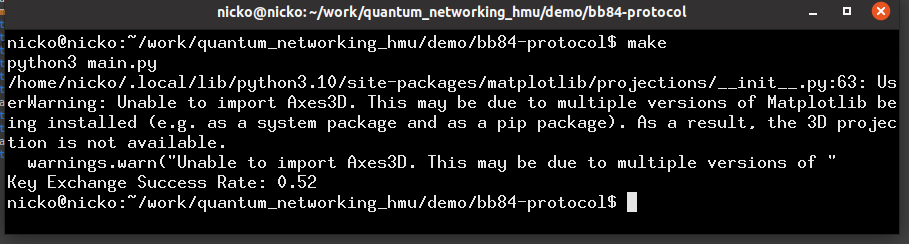
\includegraphics[width=0.7\textwidth]{bb84/success_rate_terminal.png}
			\caption{Execution of code of Listing 1 of Appendix.}
			\label{fig1:}
		\end{figure}		

		\begin{figure}[H]
			\centering
			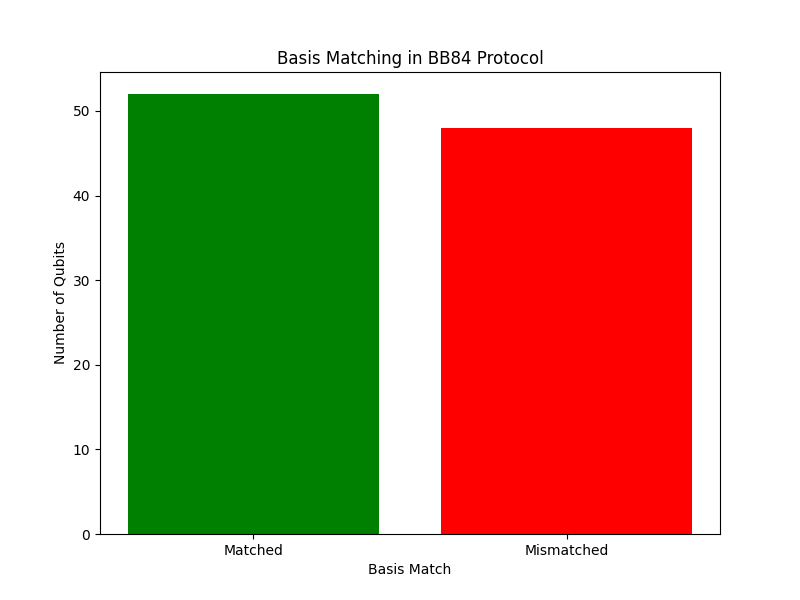
\includegraphics[width=0.6\textwidth]{bb84/basis_matching.png}
			\caption{Bases matched on the example where 100 qubits used.}
			\label{fig2:}
		\end{figure}		


		\begin{figure}[H]
			\centering
			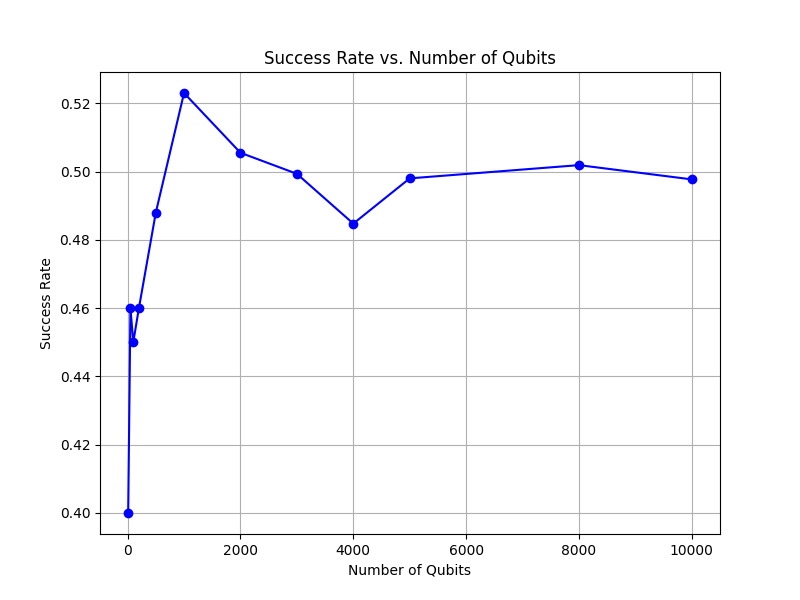
\includegraphics[width=0.6\textwidth]{bb84/success_rate_vs_num_qubits.png}
			\caption{Success rate vs number of qubits used.}
			\label{fig3:}
		\end{figure}		

		As we can observe in Figure 3, the relation of success rate is plotted against the utilized 
		number of qubits in the protocol. The simulation was run for up to 10000 qubits. 
		Success rate is converging to value 0.5, as the probability 
		of Alice and Bob choosing the same base ('x' or 'z') is 50\%.


		\subsection{QKD application using AES for classic communication}

		In the Listing 3 of Appendix, building on the previous example of generating a key,
		we extend the functionality in encrypted message exchanges among two entities, using the secret key created
		by the QKD for a symmetric encryption algorithm (in this case AES). 
		Also a limit on the success rate of the key generation is implemented,
		so each time that the success rate is not satisfied
		generation restarts. In this example 256 qubits were selected with success rate to be above 0.58.
		The execution of the simulation is presented on Figure 4, one message is sent by each entity simulating
		an encrypted ping-pong among them. In a real application we could have implemented 
		other features as well such as a key lifetime(how often the AES key should be refreshed)
		authentication between the entities start the QKD process and error correction as it would be required.
		
		\begin{figure}[H]
			\centering
			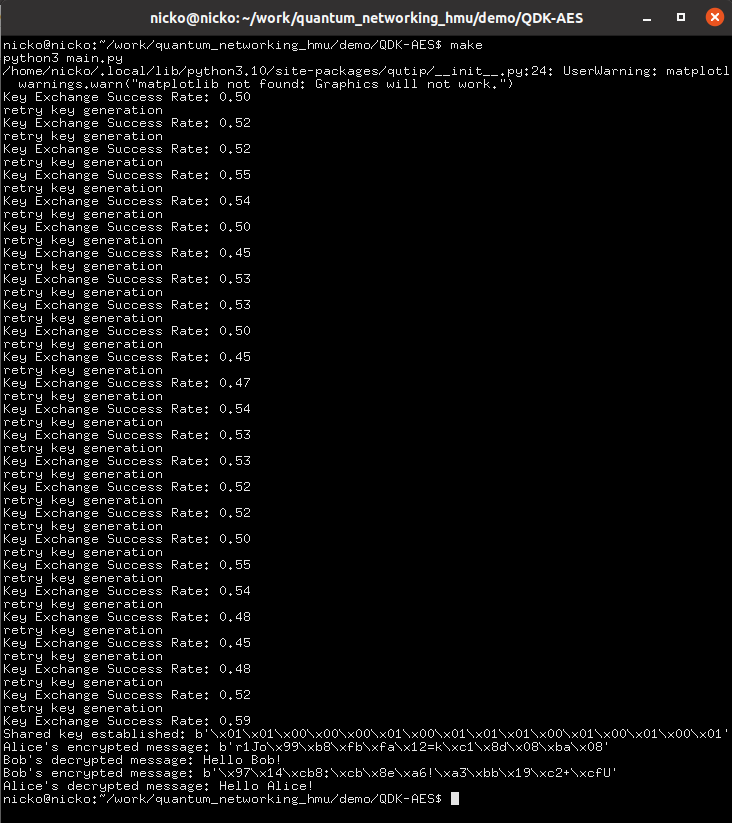
\includegraphics[width=0.7\textwidth]{qkd_aes/app.png}
			\caption{Simple encrypted message exchange among the two nodes using the key generated by QKD for AES.}
			\label{fig4:}
		\end{figure}		


		\subsection{Fidelity against Noise Level}	
		
		In this simulation (code is in Listing 2 of Appendix), a model of a quantum repeater network with
		entanglement swapping is created in order to observe how the fidelity of the final entangled state is
		affected by depolarizing noise \cite{depolarization}. Depolarizing noise is a quantum noise which models the
		coherence loss in quantum system's states because of imperfections in quantum operations.
		
		The depolarizing noise on a quantum state can be expressed as \cite{depolar2}:
			\[
			\rho \to (1-p)\rho + \frac{p}{d}I
			\]

		where:

		\begin{itemize}
			    \item \( \rho \): density matrix of quantum state before the noise is applied.
			    \item \( p \): depolarizing probability,  value \(\in [0, 1]\).
			    \item \( d \): Hilbert's space dimension. For a single qubit, \( d = 2 \).
			    \item \( I \): identity matrix \( d \times d \).
		\end{itemize}

		This form to model the noise is used in the presented simulation code.
	
		\begin{figure}[H]
			\centering
			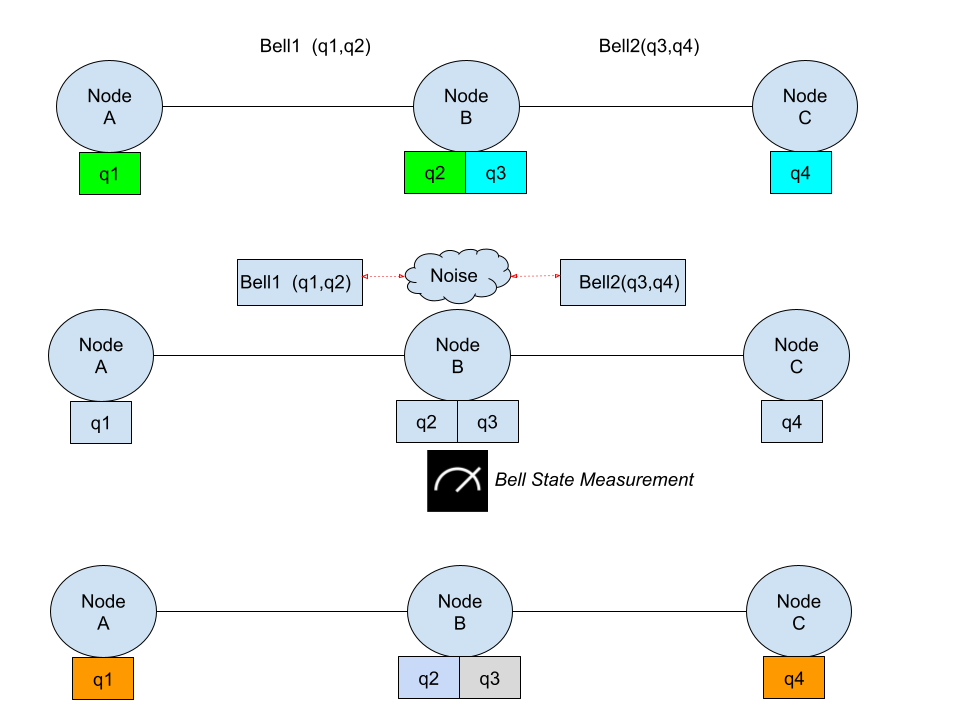
\includegraphics[width=0.6\textwidth]{repeater/entanglement_swap.png}
			\caption{Set up for the entanglement swapping}
			\label{fig5:}
		\end{figure}		

		In the set up of Figure 5 we can inspect that qubits q1 (node A) and q2 (node B) are
		entangled in Bell1(Bell state 1) and q4 (node C) and q3 (node B) are entangled in Bell2(Bell state 2).
		Node A and Node C, could create these entangled pairs and sent 1 qubit each into the intermediate
		Node B. The BSM(measurement) occurs in Node B, and as a consequence the initial entanglement between
		q3 and q4 qubits is destructed \cite{rfc}. Nevertheless the state of q2 is "recreated"/reappears in the possition
		of qubit q4, which makes an new entanglement pair consisting of qubits (q1,q4).

		Depending on the application requirements, the results of the BSM might be communicated to the Node C, in order
		to apply a correction operation on q4 depending on which Bell state was received. More specifically, the measurement
		collapses the quantum states of q2 and q3, but it also results in a change in the state of q1 and q4.
		Qubits q1 (Node A) and q4 (Node C) become entangled as a result of the BSM, but they are not measured themselves.
		This is known as the process of entanglement swapping. Now (q1,q4) share an entangled state, even though they 
		were not directly entangled initially.

		Fidelity calculates how close the state is to the desired state. 
		As the noise in the system increases, the fidelity of the final state decreases,
		indicating the decrease in quantum entanglement quality.

		\begin{figure}[H]
			\centering
			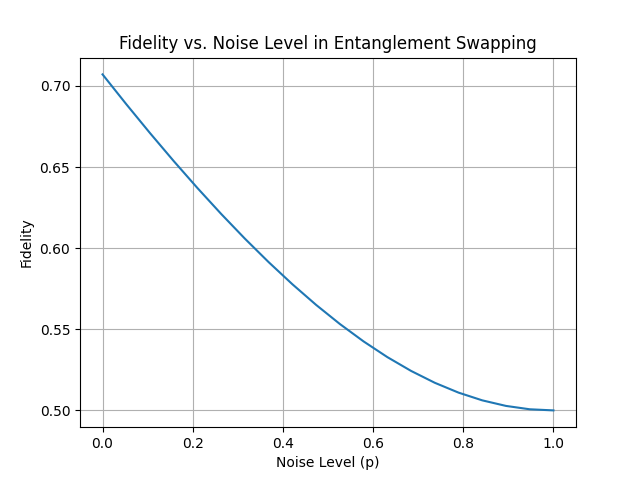
\includegraphics[width=0.5\textwidth]{repeater/fid_vs_noise.png}
			\caption{Fidelity vs Noise Level.}
			\label{fig6:}
		\end{figure}		

		A value of 1 indicates the maximum perfect fidelity where there is no loss of entanglement, 
		while lower values indicate a degradation due to noise.
		In practice a fidelity value less than 0.5 indicates that the state is unsuitable for further quantum processing.
		In Figure 6 we can inspect that as the noise level increases, the fidelity decreases,
		an expected behavior since noise disrupts the quantum states,
		making the final entangled state less similar to the ideal state.



		\subsection{Entanglement Swapping}

		For an entanglement swapping experiment, the IBM Quantum composer has been utilized for creating a circuit, which later
		was deployed in one of the available quantum processors. This experiment is actually a "continuation" from the 
		previous experiment presented in Figure 5. Again we start with 4 qubits (q[0], q[1],q[2] and q[3]) and the goal is to entangle
		q[0] and q[3]. In Figure 7 initially we create the entanglements alongside q[0] and q[1] using Hadamard gate in conjunction with
		a CNOT gate. Then the same procedure applies for qubits q[2] and q[3].

		\begin{figure}[H]
			\centering
			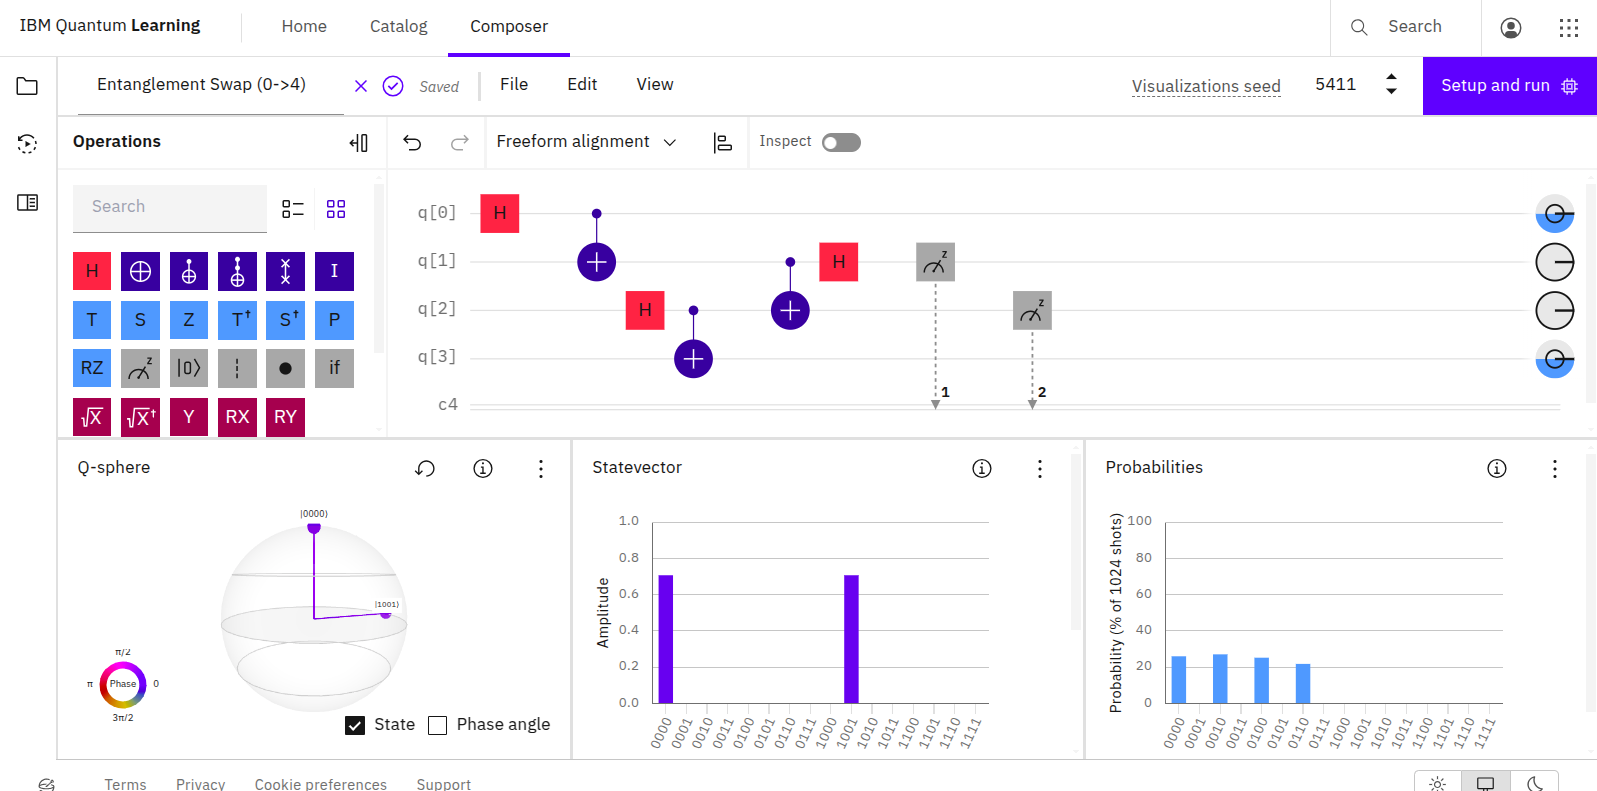
\includegraphics[width=0.6\textwidth]{ibmq/a.png}
			\caption{Design of the quantum circuit}
			\label{fig7:}
		\end{figure}		
		

		In Figure 8 we can observe on the left side of the screen the measurements of 1024 shots on the quantum processor(ibm\_sherbrook)
		the circuit was deployed and as we were expecting we have the set of the observed values(vectorstates)
		0000,0010,0010,0110 as results, stronly appearing qubits q[0] and q[3] entangled.

		\begin{figure}[H]
			\centering
			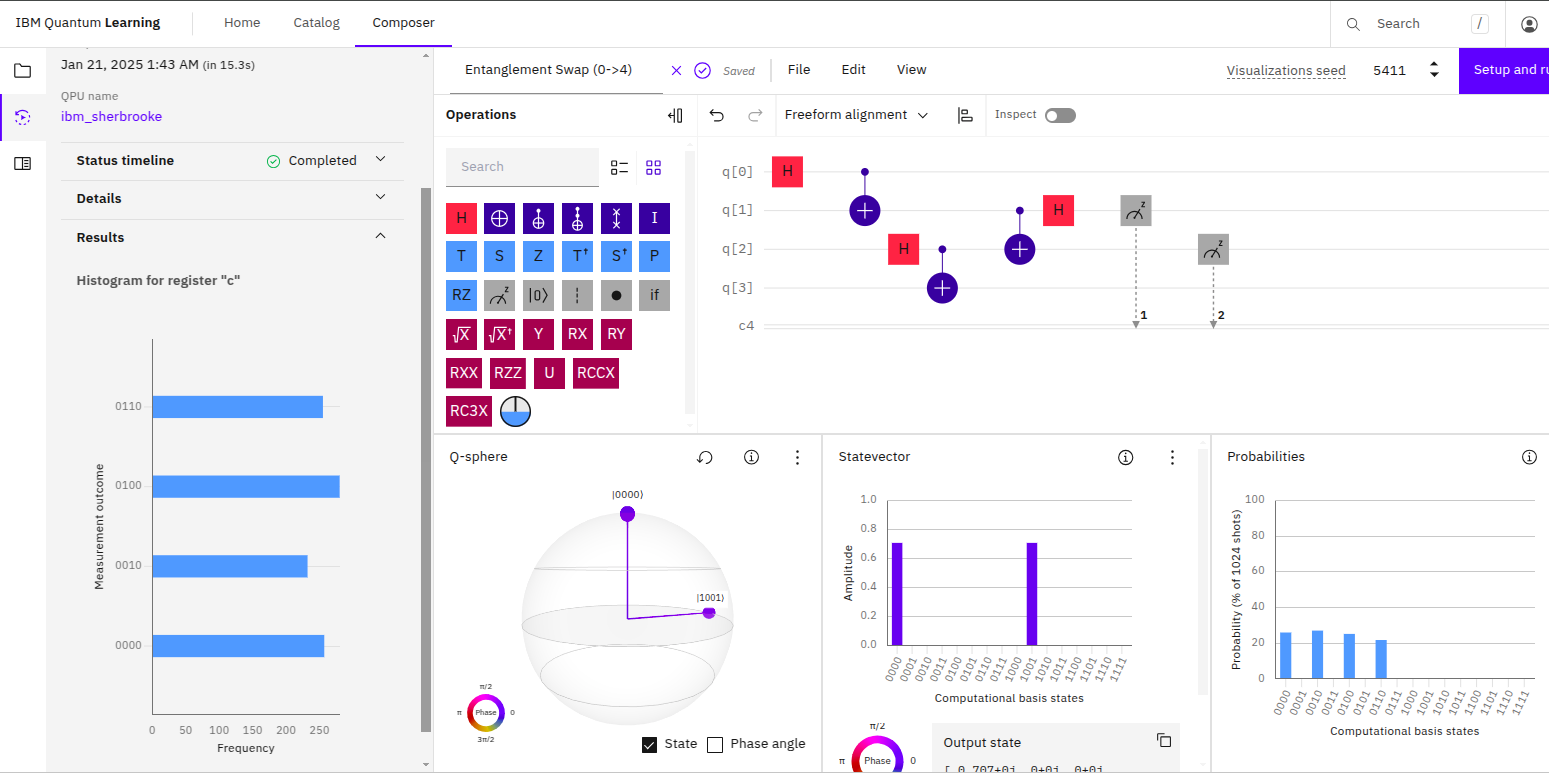
\includegraphics[width=0.6\textwidth]{ibmq/b.png}
			\caption{Left hand side of the screen depicts the results of measurement on the quantum processor}
			\label{fig8:}
		\end{figure}		
	


		Using a different circuit for the same purpose shown in Figure 9, as provided by authors in \cite{brief-intro},
		where also correction occurs conditionally based on the measured value of the qubit q[2],
		we can inspect again from the probabilities window, that the qubits q[0] and q[3] become eventually an entangled pair.

		\begin{figure}[H]
			\centering
			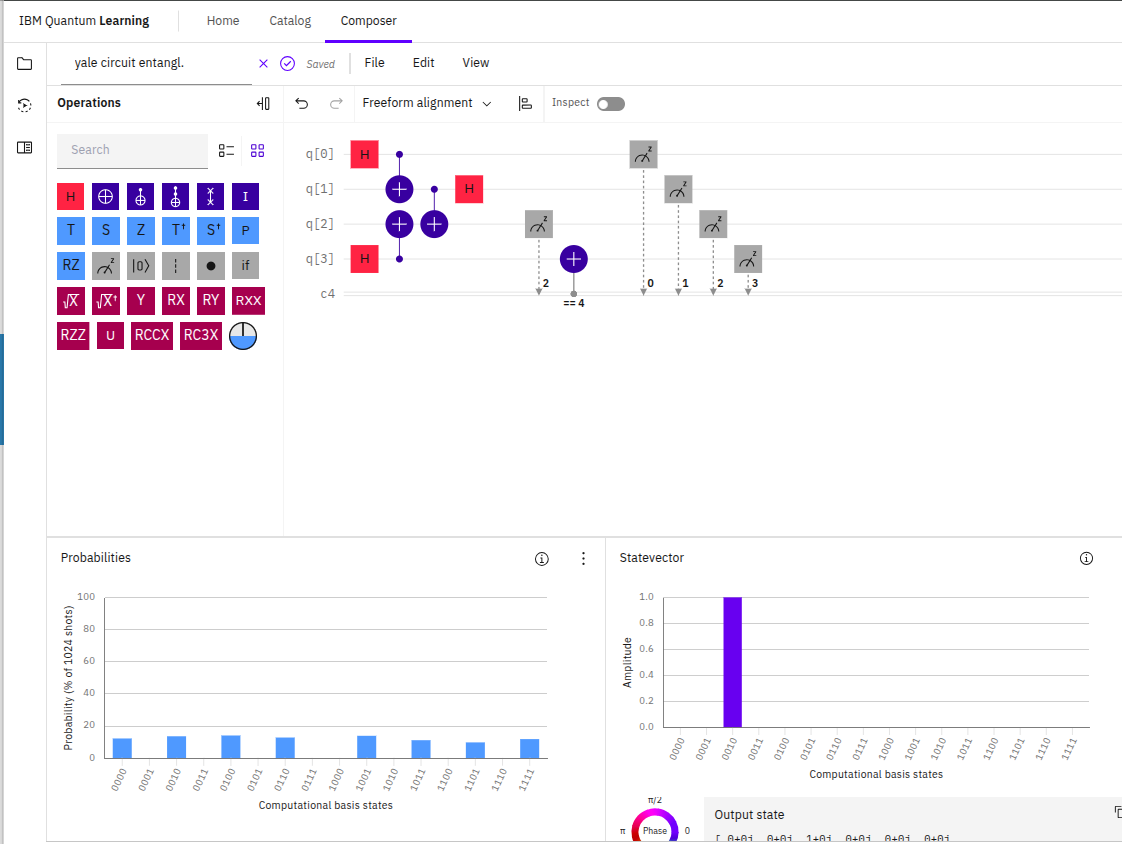
\includegraphics[width=0.6\textwidth]{ibmq/yale_circuit.png}
			\caption{Qubits q[0] and q[3] are an entangled pair}
			\label{fig9:}
		\end{figure}		
		
		When we get the results from the IBM quantum processor though, in Figure 10, we can inspect that we have 
		interference from factors that destabilize the ideal behavior of the quantum circuit, 
		and we can see the presence of combinations that we were expecting not to be present
		on the measurement.

		\begin{figure}[H]
			\centering
			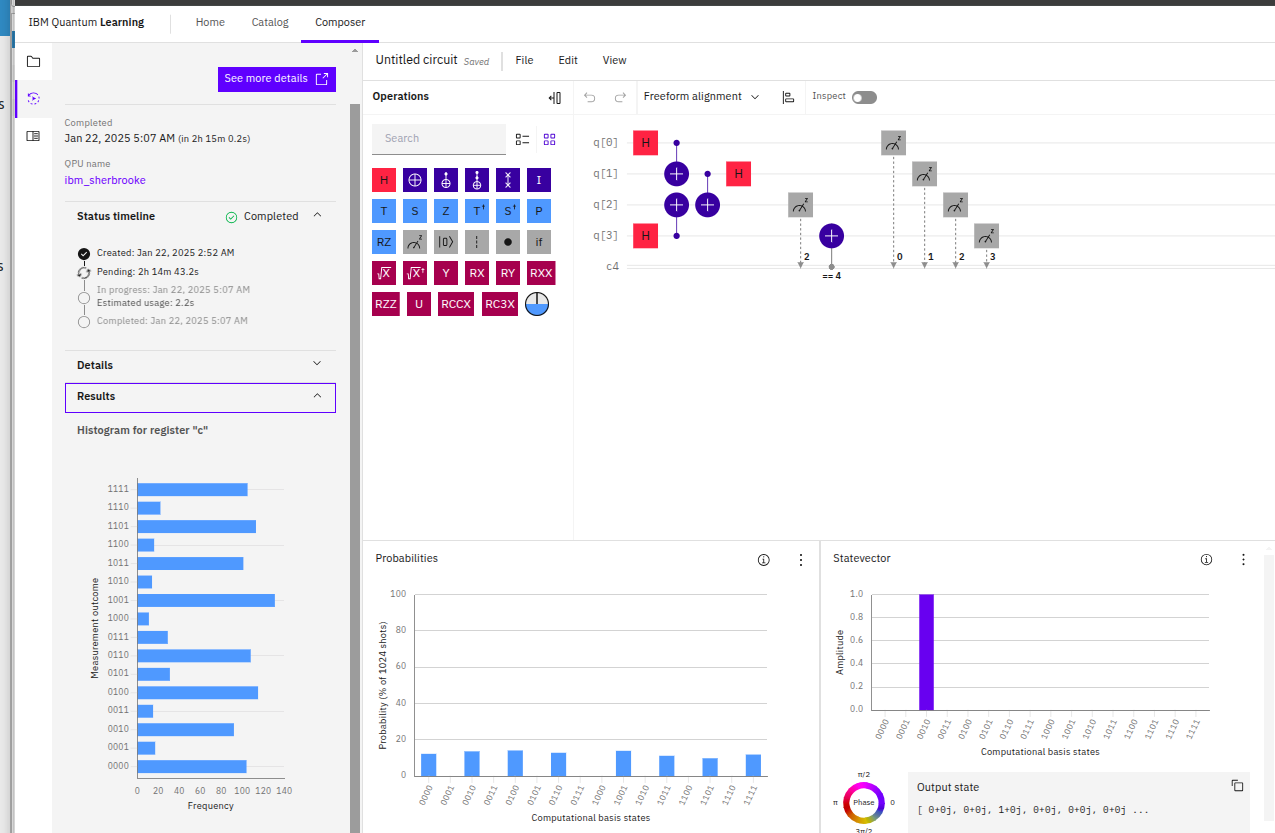
\includegraphics[width=0.6\textwidth]{ibmq/real_entanglement.png}
			\caption{Results on the left hand side, with decoherence errors from running on a real quantum processor.}
			\label{fig10:}
		\end{figure}		
		


		% noise and imperfection on measurements.
		It is important to note(Figure 11) that even in a simpler experiment with just an entangled pair on real 
		quantum processors might not perfect, and several factors can destabilize the expected states 
		(like noise, gate imperfections, readout errors, and decoherence) are present and affecting the measurements.
		As we can inspect, on the probabilities only values (00 and 11) are expected, but from the real measurements 
		on the left side of the screen we can observe mixed combinations shown up in a small ratio of the 1024 shots.
		
		\begin{figure}[H]
			\centering
			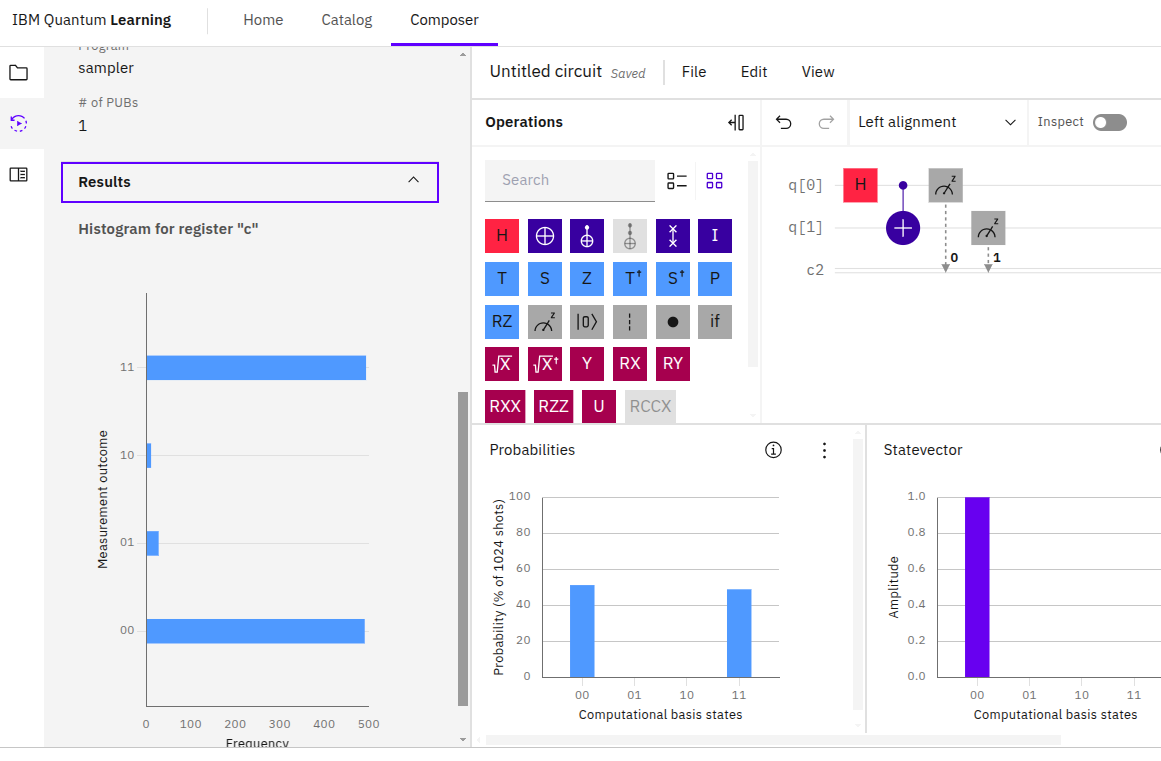
\includegraphics[width=0.6\textwidth]{ibmq/e.png}
			\caption{A simple entangled pair measurement on the quantum processor.}
			\label{fig11:}
		\end{figure}		
		
		

		\subsection{Quantum Error Correction}
		
		In this example, we have implemented the 3-qubit bit-flip code to demonstrate single-error correction in
		quantum circuits.
		In order to achieve the error correction, 3 physical qubits are encoding one logical qubit.
		For example 
		
			\[
				|1\rangle \rightarrow |111\rangle 
			\]

		Also \textit{syndrome} is used, a set of classical bits that can tell us if and where an error has
		occurred in our encoded quantum state, but without directly measuring the logical qubit itself, because
		this would result in a collapse of its state.

		Initially Figure 12, 
		we prepare the (111) state by applying the X-gate on q[0] and, 
		using CNOT with targets q[1] and q[2]
		using q[0] as control. We can observe the first 3 bits on the state vector 00\textbf{111}.
		\begin{figure}[H]
			\centering
			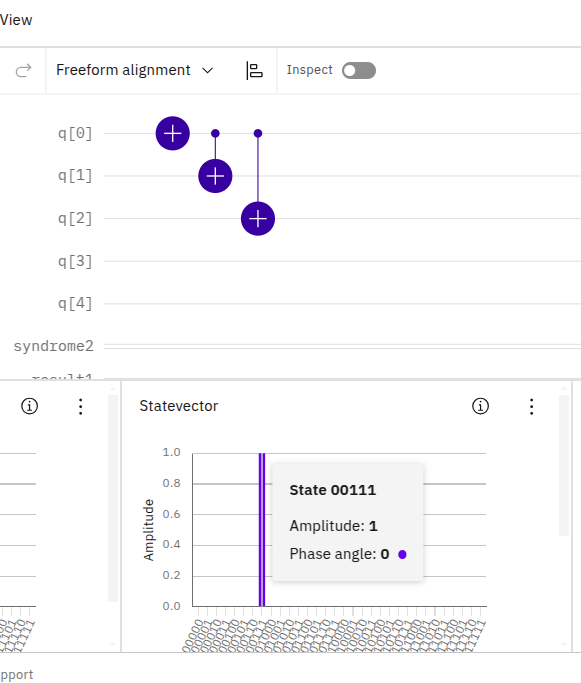
\includegraphics[width=0.3\textwidth]{ibmq/step_a.png}
			\caption{Step 1.}
			\label{fig12:}
		\end{figure}		

		Then we apply an X-gate to q[1] to introduce an error which we can observe as the 2nd bit flips
		to 00\textbf{101}(Figure 13).
		\begin{figure}[H]
			\centering
			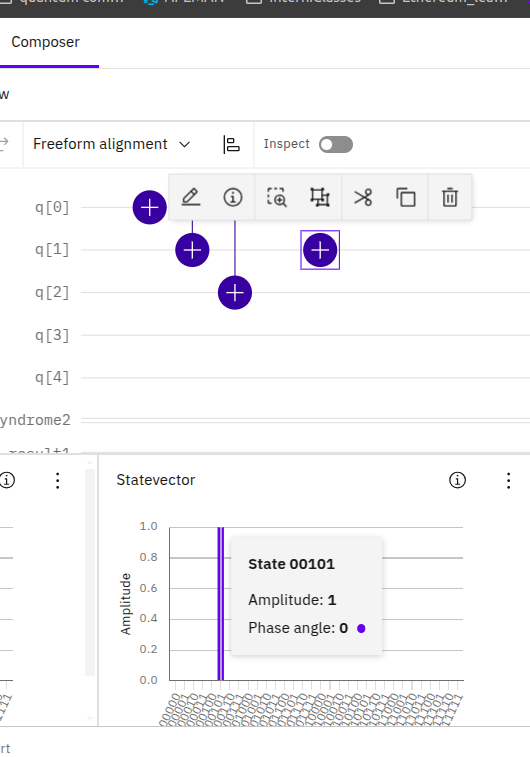
\includegraphics[width=0.3\textwidth]{ibmq/step_b.png}
			\caption{Step 2.}
			\label{fig13:}
		\end{figure}		


		In next step, we are also using the helper qubits (q[3] and q[4]) in order to detect if a 
		single bit-flip has occured without directly measuring the encoded quantum state on q[0:2] to avoid 
		state collapse.
		In first CNOT among q[0] and q[3], if q0 is 1,
		q3 flips from 0 to 1. Applying the second CNOT among q[1] and q[3], 
		if q1 is 1, q[3] flips again. In this way we compare q[0] and q[1].
		As a result, if q0 and q1 agree (both 0 or both 1), 
		q3 ends at 0 and if they do not, q[3] ends at 1.

		The same method then is repeated to compare the qubits q[1] and q[2] for aggrement.
		We take two measurements on the classical 2 bit register named \textit{syndrome}.
		As we can observe in Figure 14, all registers are showing 1's on probabilities, therefore
		\textit{syndrome} = 11, meaning as expected(because of the forced flip) 
		that both comparissons of the qubit pairs disagree and flip occured into q[1].

		\begin{figure}[H]
			\centering
			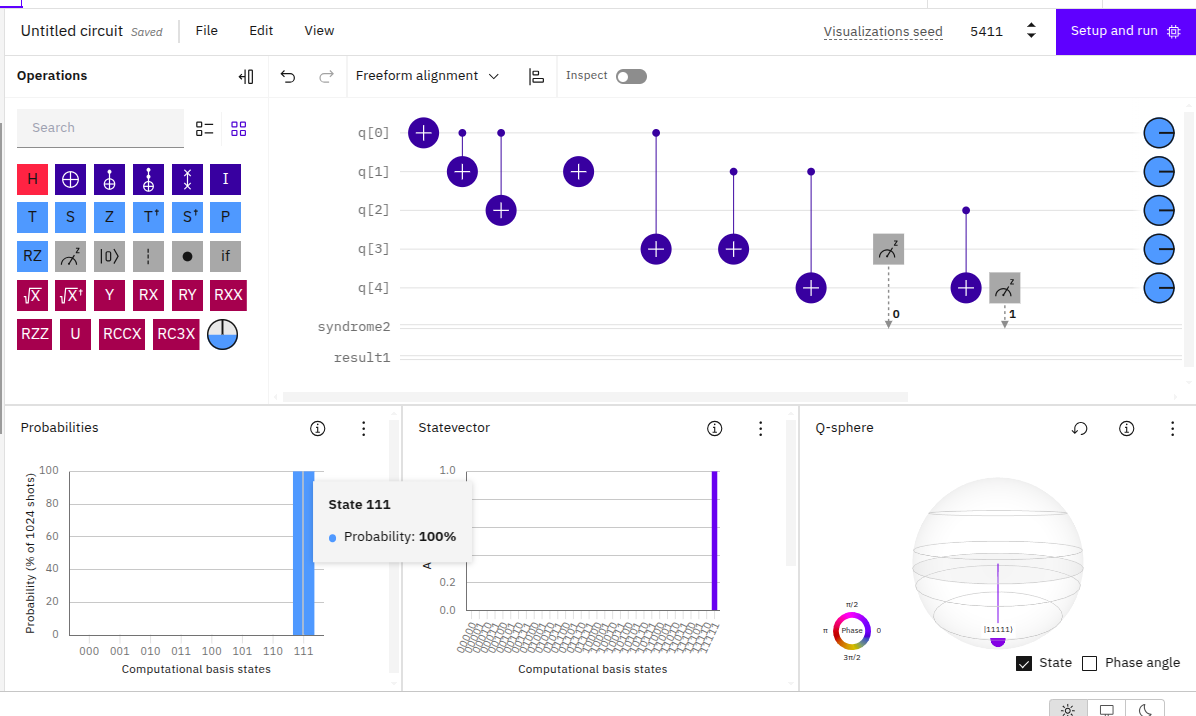
\includegraphics[width=0.5\textwidth]{ibmq/step_c.png}
			\caption{Step 3:Syndrome Measurement}
			\label{fig14:}
		\end{figure}		


		\begin{table}[ht]
		\centering
		\caption{Syndrome error locations}
		\label{tab:syndrome}
		\begin{tabular}{|c|l|}
		\hline
		\textbf{Syndrome (s[1]s[0])} & \textbf{Error Location} \\ 
		\hline
		00 & No error detected \\
		01 & Error in q2 \\
		10 & Error in q0 \\
		11 & Error in q1 \\
		\hline
		\end{tabular}
		\end{table}	

		Based on the value on the syndrome register, error correction can applied afterwards conditionally and values to be
		checked are {1,2,3}.
		Correction applied as seen in Figure 15,
		Note that in the probabilities we have a 100\% assurance that register \textit{result} should be '111'.
		\begin{figure}[H]
			\centering
			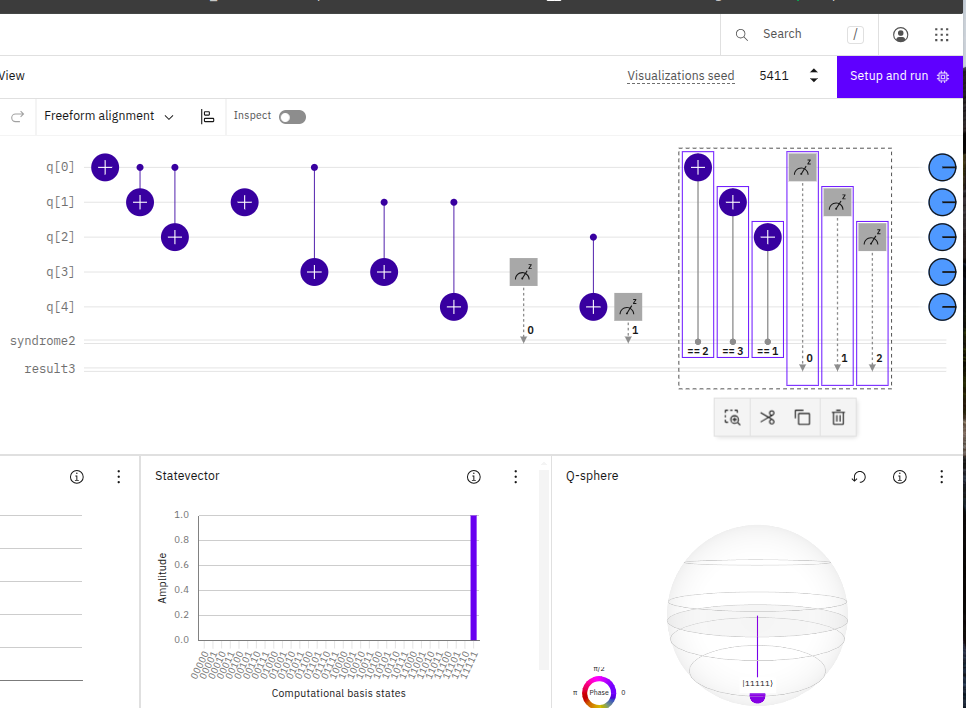
\includegraphics[width=0.5\textwidth]{ibmq/correction_circ.png}
			\caption{Correction logic for the circuit based on syndrome results.}
			\label{fig15:}
		\end{figure}		
		

		After deploying the circuit and run it for 1024 shots, on a real quantum processor offered by
		IBM, we can inspect, on the left-side of the screen that '111' was the value with the greatest probability
		of occurance for the register \textit{results} although, existing errors are observed again and differentiates the
		actual result from the simulation expected one.
		\begin{figure}[H]
			\centering
			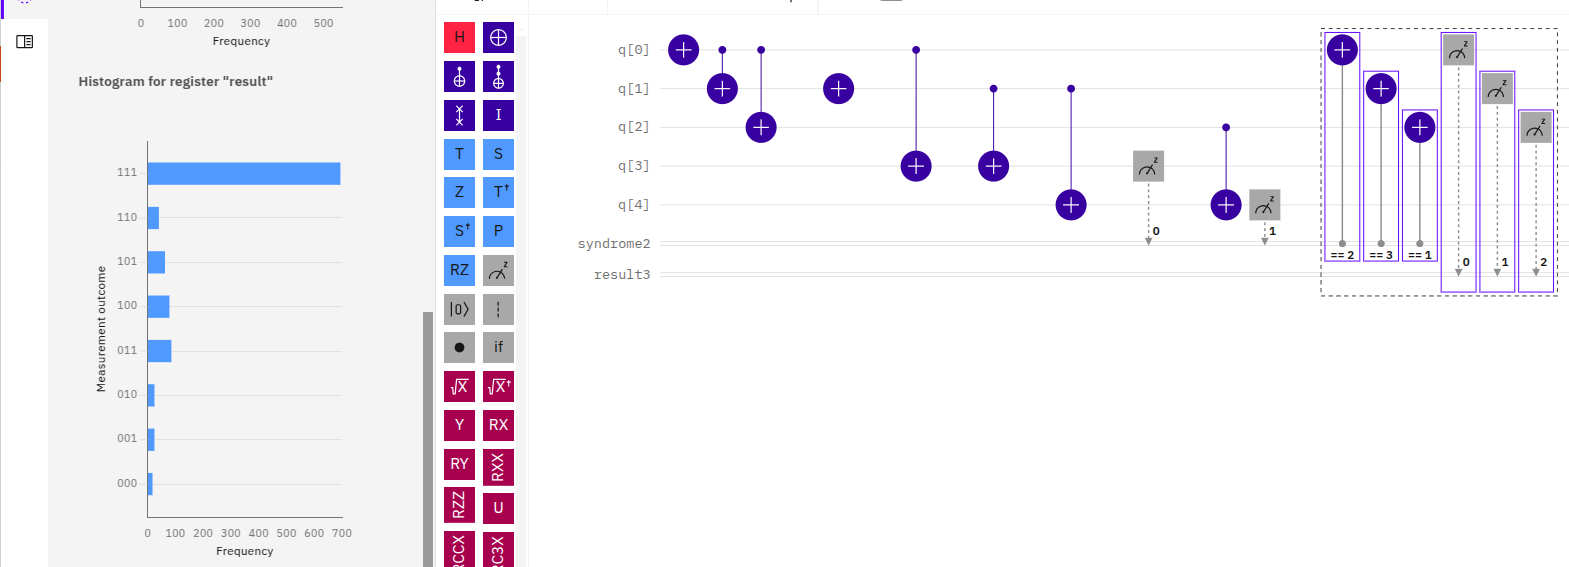
\includegraphics[width=0.6\textwidth]{ibmq/result_correction.png}
			\caption{Correction results running on IBMQ quantum processor.}
			\label{fig15:}
		\end{figure}		
		
		The auto-generated Qiskit code for the 3 qubit single bit flip error correection code is presented on
		Appenix A's Listing 4.

	\section{Discussion}
	

	The simulations and experiments presented in the previous section can provide insights into the practical implementation 
	of quantum networking protocols and the challenges arising by the real world quantum hardware. 

	\textit{1. BB84 protocol}
	\newline
	The convergence of the BB84 protocol’s success rate to ~50\% (Figure 3) agrees with the theoretic probability 
	of Alice and Bob of choosing matching bases. 
	In practical deployments, increasing the number of qubits ensures a longer secret key, 
	although that will demand also increased error corrections to tackle losses and ensure higher fidelities and keeping stable the entanglements.
	

	\textit{2. QKD-AES example}
	\newline
	The integration of QKD with AES (Figure 4) demonstrates the hybrid approach of secure communication, 
	after having established a secret key among the entities with a threshold rate.
	In real-world scenarios, dynamic threshold adjustments on the success rate could be implemented to
	optimize performance under varying network environments. 
	

\textit{3. Fidelity Degradation in Noisy Quantum Repeaters}
	\newline
	The relationship between depolarizing noise and fidelity appearing in the graph(Figure 6) denotes the challenge of long distance quantum networks. 
	In any case, fidelity never should drop below 0.5, rendering the entangled states unsuitable for quantum protocols. 
	This emphasizes the need for having available low noise repeaters,
	deployment of error correction and entanglement purification schemes in order to keep fidelity in desired high levels.

\textit{4. Entanglement Swapping on Real Quantum Hardware}
	\newline
	The entanglement swapping experiments (Figures 7–11) shows the differences from theoretic expectations and what real device outputs. 
	While simulations (Figures 7–9) can show perfect entanglement, IBM Quantum results (Figures 10–11) experience some decoherence errors 
	(f.e, unexpected states like (01),(01)), highlighting some limitations and deviation from the ideal measurement on current devices. 
	These errors arise from gate imperfections and readout errors, and shows the need of more advanced error tackling techniques.

\textit{5. Quantum Error Correction on Real Hardware}
	\newline
	The 3-qubit bit flip code (Figures 12–15) successfully corrected single-qubit errors in simulation 
	but showed some errors on IBMQ hardware. 
	The percentage of success rate of the experiment(Figure 15) reflects the effects of gate and readout errors. 
	Also in order to be able of detecting flips on more than a single qubit, 
	larger quantum circuits are required(5-qubit or 9-qubit) which also introduces
	more gate-related noise on the circuit.

\section{Conclusion}

	In this project we have explored quantum networking protocols like BB84 and entanglement swapping while introduced to hardware 
	limitations of the current available quantum processors. 
	As quantum hardware keeps maturing with combination of better and more efficient error corrections, low-noise repeaters, 
	and hybrid quantum-classical systems, the path will lead into more secure quantum networks and a complete architecture.

\newpage
\bibliographystyle{plain}
\bibliography{references}
\newpage
\appendix

\section{Appendix A: Simulation Code }

%\begin{lstlisting}[language=Python, caption=BB84 for QKD, label=code:QKD, escapeinside=||]
\begin{lstlisting}[language=Python, caption=BB84 for QKD, label=code:QKD]
from qutip import basis, ket2dm
import numpy as np
zero = basis(2, 0)  ''' |0> '''
one = basis(2, 1)   ''' |1> ''' 
plus = (zero + one).unit()  ''' |+> '''
minus = (zero - one).unit() ''' |-> ''' 
''' Alice's qubits'''
def generate_bb84_states(num_qubits):
    states = []
    bases = []
    for _ in range(num_qubits):
        basis_choice = np.random.choice(['z', 'x'])
        bit = np.random.choice([0, 1])
        if basis_choice == 'z':
            states.append(zero if bit == 0 else one)
        else:
            states.append(plus if bit == 0 else minus)
        bases.append(basis_choice)
    return states, bases
'''Measurement'''
def measure_state(state, basis):
    if basis == 'z':
        projection = [zero, one]
    else:  ''' 'x' '''
        projection = [plus, minus]
    probabilities = [abs(proj.overlap(state))**2 for proj in projection]
    return np.random.choice([0, 1], p=probabilities)
'''Simulation'''
num_qubits = 100
alice_states, alice_bases = generate_bb84_states(num_qubits)
bob_bases = np.random.choice(['z', 'x'], num_qubits)
''' Measure and compare '''
bob_results = [measure_state(state, bob_bases[i]) for i, state in enumerate(alice_states)]
matching_bases = [alice_bases[i] == bob_bases[i] for i in range(num_qubits)]
shared_key = [bob_results[i] for i in range(num_qubits) if matching_bases[i]]
''' Calculate success rate'''
success_rate = len(shared_key) / num_qubits
print(f"Key Exchange Success Rate: {success\_rate:.2f}")
import matplotlib.pyplot as plt
''' Visualization 1: Basis Matching (Bar Chart)'''
matched = sum(matching_bases)
mismatched = num_qubits - matched
plt.figure(figsize=(8, 6))
plt.bar(['Matched', 'Mismatched'], [matched, mismatched], color=['green', 'red'])
plt.title('Basis Matching in BB84 Protocol')
plt.xlabel('Basis Match')
plt.ylabel('Number of Qubits')
plt.savefig('Basis Matching in BB84 Protocol.png')
''' Visualization 2: Success Rate vs. Number of Qubits (Line Chart) '''
num_qubits_list = [10, 50, 100, 200, 500, 1000, 2000, 3000, 4000, 5000, 8000, 10000]
success_rates = []
for nq in num_qubits_list:
    alice_states, alice_bases = generate_bb84_states(nq)
    bob_bases = np.random.choice(['z', 'x'], nq)
    bob_results = [measure_state(state, bob_bases[i]) for i, state in enumerate(alice_states)]
    matching_bases = [alice_bases[i] == bob_bases[i] for i in range(nq)]
    shared_key = [bob_results[i] for i in range(nq) if matching_bases[i]]
    success_rate = len(shared_key) / nq
    success_rates.append(success_rate)
plt.figure(figsize=(8, 6))
plt.plot(num_qubits_list, success_rates, marker='o', color='b')
plt.title('Success Rate vs. Number of Qubits')
plt.xlabel('Number of Qubits')
plt.ylabel('Success Rate')
plt.grid(True)
plt.savefig("Success Rate vs Number of Qubits.png")

\end{lstlisting}


\begin{lstlisting}[language=Python, caption=Entanglement swapping(fidelity vs polarizing noise), label=code:entanglement-swap]

from qutip import *
import numpy as np
import matplotlib.pyplot as plt

''' Define Bell state '''
def create_bell_state():
    zero = basis(2, 0)  
    one = basis(2, 1)   
    bell_state = (tensor(zero, zero) + tensor(one, one)).unit()  
    bell_dm = ket2dm(bell_state)  ''' Convert to density matrix, shape: (4, 4)'''
    return bell_dm

''' Apply noise to a quantum state (Depolarizing channel)'''
def apply_depolarizing_noise(state, p):
    dim = np.prod(state.dims[0])  ''' Total dimension of the system'''
    identity = qeye(dim)  ''' Identity operator, shape: (dim, dim)'''
    identity.dims = state.dims
    n1=(1-p)*state
    n2 = (p/dim)*identity
    noisy_state = (1 - p) * state + (p / dim) * identity
    return noisy_state

''' Entanglement swapping '''
def entanglement_swapping(bell1, bell2):
    """
    Perform entanglement swapping between two Bell states:
    bell1: A-B (shape: (4, 4)), bell2: B-C (shape: (4, 4))
    Returns:
    - swapped_state: final entangled state between A and C (shape: (4, 4))
    """
    # Bell measurement on qubits 2 and 3 (middle qubits)
    bell_meas = (tensor(basis(2, 0), basis(2, 0)).proj() + 
                 tensor(basis(2, 1), basis(2, 1)).proj())  # Bell basis, shape: (4, 4)
    projection = tensor(qeye(2), bell_meas, qeye(2))  # Operate on qubits 2 and 3, shape: (16, 16)
    
    # Combine the two input states into a joint density matrix
    joint_state = tensor(bell1, bell2)  # Combined state, shape: (16, 16)
    
    # Apply projection for entanglement swapping
    swapped_state = (projection * joint_state * projection.dag()).unit()  # Shape: (16, 16)
    
    # Partial trace over qubits 2 and 3 to get A-C state
    final_state = swapped_state.ptrace([0, 3])  # Shape: (4, 4)
    return final_state

# Network Simulation
def simulate_network():
    """
    Simulates a basic quantum repeater network with entanglement swapping.
    Returns:
    - fidelity_value: fidelity of the final entangled state with an ideal Bell state
    """
    noise_levels = np.linspace(0, 1, 20)  # Noise levels from 0 to 1
    fidelities = []


    ''' Step 1: Create initial entanglement between nodes'''
    bell1 = create_bell_state()  # Between nodes A and B
    print(bell1)

    bell2 = create_bell_state()  # Between nodes B and C
    print(bell2)
    
    ''' Step 2: Calculate fidelity for different noise levels '''
    for p in noise_levels:
        bell1_noisy = apply_depolarizing_noise(bell1, p)
        bell2_noisy = apply_depolarizing_noise(bell2, p)
        final_state = entanglement_swapping(bell1_noisy, bell2_noisy)
        ideal_bell = create_bell_state()
        print(ideal_bell)
        fidelity_value = fidelity(final_state, ideal_bell)
        fidelities.append(fidelity_value)
    
    ''' Step 3: Plot fidelity vs noise level'''
    plt.plot(noise_levels, fidelities)
    plt.xlabel("Noise Level (p)")
    plt.ylabel("Fidelity")
    plt.title("Fidelity vs. Noise Level in Entanglement Swapping")
    plt.grid(True)
    plt.savefig("Fidelity vs Noise Level in Entanglement Swapping.png")   

# Main Execution
if __name__ == "__main__":
    simulate_network()

\end{lstlisting}

\begin{lstlisting}[language=Python, caption= QKD-AES application, label=code:QKD]

from qutip import basis, ket2dm
import numpy as np
from Crypto.Cipher import AES
from Crypto.Util.Padding import pad, unpad
import os

# Define basis states of computational basis and Hadamard basis
zero = basis(2, 0)  # |0>
one = basis(2, 1)   # |1>
plus = (zero + one).unit()  # |+>
minus = (zero - one).unit()  # |->

# Alice's qubits
def generate_bb84_states(num_qubits):
    states = []
    bases = []
    for _ in range(num_qubits):
        basis_choice = np.random.choice(['z', 'x'])
        bit = np.random.choice([0, 1])
        if basis_choice == 'z':
            states.append(zero if bit == 0 else one)
        else:
            states.append(plus if bit == 0 else minus)
        bases.append(basis_choice)
    return states, bases

# Measurement
def measure_state(state, basis):
    if basis == 'z':
        projection = [zero, one]
    else:  # 'x'
        projection = [plus, minus]
    probabilities = [abs(proj.overlap(state))**2 for proj in projection]
    return np.random.choice([0, 1], p=probabilities)

# Generate shared key
def generate_shared_key(num_qubits):
    alice_states, alice_bases = generate_bb84_states(num_qubits)
    bob_bases = np.random.choice(['z', 'x'], num_qubits)

    # Bob measures Alice's qubits
    bob_results = [measure_state(state, bob_bases[i]) for i, state in enumerate(alice_states)]
    matching_bases = [alice_bases[i] == bob_bases[i] for i in range(num_qubits)]
    shared_key = [bob_results[i] for i in range(num_qubits) if matching_bases[i]]

    # Success rate
    success_rate = len(shared_key) / num_qubits
    print(f"Key Exchange Success Rate: {success_rate:.2f}")

    # Ensure we have a sufficiently long key for AES (128 bits = 16 bytes)
    if len(shared_key) >= 16:
        shared_key = shared_key[:16]
        return bytes(shared_key), success_rate
    else:
        print("Not enough key bits generated. Increase number of qubits.")
        return None, success_rate

# Encrypt and decrypt messages using AES
def encrypt_message(message, key):
    cipher = AES.new(key, AES.MODE_CBC)  # Use AES in CBC mode
    iv = cipher.iv
    encrypted_message = cipher.encrypt(pad(message.encode(), AES.block_size))
    return iv, encrypted_message

def decrypt_message(iv, encrypted_message, key):
    cipher = AES.new(key, AES.MODE_CBC, iv=iv)
    decrypted_message = unpad(cipher.decrypt(encrypted_message), AES.block_size)
    return decrypted_message.decode()

# Main simulation
num_qubits = 256
success_rate = 0
RATE = 0.57
while(success_rate <= RATE):
    key, success_rate = generate_shared_key(num_qubits)
    if(success_rate < RATE):
        print("retry key generation")

if key and success_rate > RATE:  # Use the key if success rate is high enough
    print("Shared key established:", key)

    # Alice sends a message to Bob
    alice_message = "Hello Bob!"
    iv, encrypted_message = encrypt_message(alice_message, key)
    print(f"Alice's encrypted message: {encrypted_message}")

    # Bob decrypts the message
    bob_message = decrypt_message(iv, encrypted_message, key)
    print(f"Bob's decrypted message: {bob_message}")

    # Bob sends a message to Alice
    bob_message = "Hello Alice!"
    iv, encrypted_message = encrypt_message(bob_message, key)
    print(f"Bob's encrypted message: {encrypted_message}")

    # Alice decrypts the message
    alice_message = decrypt_message(iv, encrypted_message, key)
    print(f"Alice's decrypted message: {alice_message}")
else:
    print("Failed to generate a secure shared key.")

\end{lstlisting}

\begin{lstlisting}[language=Python, caption= 3 qubit single bit flip error correction circuit, label=code:QKD]
from qiskit import QuantumRegister, ClassicalRegister, QuantumCircuit
from numpy import pi
qreg_q = QuantumRegister(5, 'q')
creg_syndrome = ClassicalRegister(2, 'syndrome')
creg_result = ClassicalRegister(3, 'result')
circuit = QuantumCircuit(qreg_q, creg_syndrome, creg_result)
circuit.x(qreg_q[0])
circuit.cx(qreg_q[0], qreg_q[1])
circuit.cx(qreg_q[0], qreg_q[2])
circuit.x(qreg_q[1])
circuit.cx(qreg_q[0], qreg_q[3])
circuit.cx(qreg_q[1], qreg_q[3])
circuit.cx(qreg_q[1], qreg_q[4])
circuit.measure(qreg_q[3], creg_syndrome[0])
circuit.cx(qreg_q[2], qreg_q[4])
circuit.measure(qreg_q[4], creg_syndrome[1])
circuit.x(qreg_q[0]).c_if(creg_syndrome, 2)
circuit.x(qreg_q[1]).c_if(creg_syndrome, 3)
circuit.x(qreg_q[2]).c_if(creg_syndrome, 1)
circuit.measure(qreg_q[0], creg_result[0])
circuit.measure(qreg_q[1], creg_result[1])
circuit.measure(qreg_q[2], creg_result[2])
# @columns [0,1,2,4,6,8,10,12,14,15,17,18,19,20,21,22]
\end{lstlisting}

\end{document}
